\documentclass[../main.tex]{subfiles}

\begin{document}

\chapter{Die Geometrie der Gaussabbildung}

\section{Gaussabbildung}


%% For figures without text: 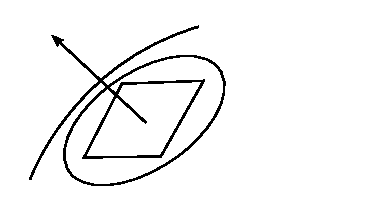
\includegraphics[width=8em]{figures/Einheitsnormalenfeld.pdf}

\begin{minipage}{0.7\columnwidth}
    \begin{definition}
        Sei $\Sigma \subset \mathbb{R}^{3}$ eine reguläre Fläche und $V \subset \Sigma$ offen. Eine stetige Abbildung $N:V \to S^2$ heisst \emph{Einheitsnormalenfeld} (oder lokale Gaussabbildung), falls für alle $p \in V$ gilt
        \begin{align*}
            N(q)\perp T_{p}\Sigma
        \end{align*}
    \end{definition}
\end{minipage}
\hspace{0.05\linewidth}
\begin{minipage}{0.3\columnwidth}
    \begin{figure}[H]
        \centering
        \def\svgwidth{\textwidth}
        \input{figures/Einheitsnormalenfeld.pdf_tex}
        \caption*{Einheitsnormalenfeld}        
    \end{figure}
\end{minipage}

\begin{existence}
    Definiere
    \begin{align*}
        N : V & \to S^{2} \\
        q & \mapsto \frac{\varphi_{u}(q) \times \varphi_{v}(q)}{\lVert \varphi_{u}(q) \times \varphi_{v}(q) \rVert_{2}}
    \end{align*}
    Dieser Ausdruck ist stetig in $q$, da $\varphi_{u}$ und $\varphi_{v}$ stetig sind.
\end{existence}
\begin{uniqueness}
    Falls $V$ zusammenhängend ist, dann ist $N:V \to S^{2}$ bis auf Vorzeichen eindeutig festgelegt $:\pm N$.
\end{uniqueness}
\begin{remark}
    Falls $\Sigma \subset \mathbb{R}^{3}$ geschlossen ist (d.h. kompakt und ohne Rand), dann existiert sogar ein globales Einheitsnormalenfeld $N:\Sigma \to S^{2}$, genannt \emph{Gaussabbildung}.
    Tatsächlich trennt eine solche Fläche $\mathbb{R}^{3}$ in zwei Zusammenhangskomponenten. Für (nicht-geschlossene) reguläre Fläche $\Sigma \subset \mathbb{R}^{3}$ gilt: Es existiert $N:\Sigma \to S^{2}$ stetiges Einheitsnormalenfeld genau dann,
    wenn $\Sigma$ \emph{orientierbar} ist.
\end{remark}
\begin{figure}[H]
    \centering
    \def\svgwidth{\textwidth}
    \input{figures/Orientierbarkeit.pdf_tex}
    \caption*{orientierbarer Brezel, Möbiusband ist nicht orientierbar}        
\end{figure}

Sei nun $\varphi : U \to V \subset \Sigma$ eine lokale $C^{1}$-Parametrisierung und $N:V \to S^{2}$ eine lokale Gaussabbildung. Dann gilt für alle $q \in V$:


\begin{itemize}
    \item $N(q) \perp T_{q}\Sigma$
    \item $N(q) \perp T_{N(q)}S^{2}$
\end{itemize}
Wir schliessen (da in $\mathbb{R}^3$): $$T_{q}\Sigma = T_{N(q)}S^{2}$$
Bei letzterem gilt also für alle $ p \in S^{2}: p\perp T_{p}S^2$.
Falls $N:V \to S^{2}$ sogar differenzierbar ist, dann erhalten wir für alle $ p \in V$ eine Abbildung
\begin{align*}
    (DN)_{p}: T_{p}\Sigma \to T_{N(p)}S^{2} = T_{p}\Sigma    
\end{align*}
die \emph{Weingartenabbildung}.

\begin{definition}$K(p) = \det{(DN)_{p}}\in \mathbb{R}$. Die \emph{Gausssche Krümmung} im Punkt $p \in \Sigma$
\end{definition}

\begin{remark}
    $K(p)$ hängt nicht von der Wahl von $N$ ab, da $$\det(-(DN)_{p}) = (-1)^{2} \det(DN)_{p}$$
\end{remark}
\begin{examples}
    \leavevmode
    \begin{enumerate}
        \item 
        \begin{minipage}[t]{0.6\columnwidth}
            $\Sigma = \mathbb{R}^{2} \times \{0\} \subset \mathbb{R}^{3}$
            \begin{align*}
                N : \Sigma & \to S^{2}\\
                q & \mapsto e_{3} \qquad \text{(oder$-e_{3}$)}\\
            \end{align*}
        \end{minipage}
        \begin{minipage}[t]{0.2\columnwidth}
            \begin{figure}[H]
                \centering
                \def\svgwidth{\textwidth}
                \input{figures/kruemmung_ebene.pdf_tex}
            \end{figure}
        \end{minipage}

        $N$ ist konstant, also gilt für alle $q \in \Sigma$: $(DN)_{q} = 0, K(q) = 0$.
        \newpage

        \item 

        \begin{minipage}[t]{0.6\columnwidth}
            $\Sigma = S^{2} \subset \mathbb{R}^{3}$ (Einheitssphäre)
            \begin{align*}
                N: S^{2} &\to S^{2}\\
                q &\mapsto q
            \end{align*}
        \end{minipage}
        \begin{minipage}[t]{0.2\columnwidth}
            \begin{figure}[H]
                \centering
                \def\svgwidth{\textwidth}
                \input{figures/kruemmung_kugel.pdf_tex}
            \end{figure}
        \end{minipage}

        $N = Id_{S^{2}}$ (oder $-Id_{S^{2}}$), für alle $q \in S^{2}$ gilt also $(DN)_{q} = Id : T_{q}\Sigma \to T_{q}\Sigma$.
        Also $K(q) = \det (Id: T_{q}\Sigma \to T_{q}\Sigma) = 1$


        \item 

        \begin{minipage}[t]{0.6\columnwidth}
            $Z = \{ (x,y,z)\in \mathbb{R}^{3} \ | \ x^{2} + y^{2} = 1 \}\subset \mathbb{R}^3 $
            \begin{align*}
                N : Z &\to S^{2}\\
                (x,y,z) &\mapsto (x,y,0)
            \end{align*}
        \end{minipage}
        \begin{minipage}[t]{0.2\columnwidth}
            \begin{figure}[H]
                \centering
                \def\svgwidth{\textwidth}
                \input{figures/kruemmung_zylinder.pdf_tex}
            \end{figure}
        \end{minipage}

        Wir bemerken: $N$ hängt nicht von $z$ ab. 
        Also gilt für alle $q \in Z$ : $$(DN)_{q}(e_{3}) = \lim\limits_{t \rightarrow 0}{\frac{\overbrace{N(q + t \cdot e_{3}) - N(q)}^{=0}}{t}} = 0$$\\
        $\implies 0$ ist ein Eigenwert der Abbildung $(DN)_{q} : T_{q}Z \to T_{q}Z \implies K(q) = 0$.
    \end{enumerate}
    \begin{zusatz}
        Genauere Betrachtung des dritten Beispiels:
        Für $q = (x,y,z) \in Z$ gilt: $$T_{q}Z = \text{span}\{e_{3}, \overbrace{-y \cdot e_{1} + x \cdot e_{2}}^{v}\}$$
        Wir bestimmen $(DN)_{q}\stackrel{(\text{*})}{=} v$.
        (*) Erklärung: Die Einschränkung von $N$ auf $S^1\times \{0\}$ ist die Identität. Folglich ist die Abbildungsmatrix von $(DN)_{q}$ bezüglich der Basis $\{ e_{3}, -y e_{1} + x e_{2} \}$
    \end{zusatz}
\end{examples}
\begin{definition}
    Die \emph{mittlere Krümmung} im Punkt $p \in \Sigma$ ist $H(p) = \frac{1}{2} \text{Spur}((DN)_{p})\in \mathbb{R}$, welche allerdings nur bis auf Vorzeichen definiert ist:
    $\text{Spur}(-(DN)_{p}) = - \text{Spur}(DN)_{p}$

\end{definition}
\begin{remark}
    Reguläre Flächen mit $H \equiv 0$ heissen \emph{Minimalflächen}.
\end{remark}

\begin{examples}
    \leavevmode
    \begin{enumerate}
       \item $\Sigma = \mathbb{R}^{2} \times \{0\}$ \qquad $K\equiv 0$ und $H\equiv 0$.
       \item $\Sigma = S^{2}$\qquad $K \equiv 1 \text{ und } H\equiv 1 \impliedby \frac{1}{2}\text{ Spur}\begin{pmatrix}
           1 & 0 \\
           0 & 1
       \end{pmatrix}$
       \item $\Sigma = Z$\qquad $K\equiv 0$ und $H\equiv \frac{1}{2} \impliedby \frac{1}{2} \cdot (\underbrace{\lambda_{1}}_{EW_{1}} + \underbrace{\lambda_{2}}_{EW_{2}}) = \frac{1}{2} \cdot (1 + 0)$ 
    \end{enumerate}
\end{examples}

\begin{notation}
    Ein Punkt $p\in \Sigma$ heisst: \\
    \begin{minipage}[c][10em]{0.7\columnwidth}
            \begin{itemize}
                \item \emph{elliptisch}, falls $K(p) > 0$
                \item \emph{hyperbolisch}. falls $K(p) < 0$ (Sattelpunkt, siehe später)
                \item \emph{parabolisch}, falls $K(p) = 0 \text{ und } H(p) \neq 0$
                \item \emph{Flachpunkt}, falls $K(p) = 0 \text{ und } H(p) = 0$
            \end{itemize}
    \end{minipage}
    \begin{minipage}[c][10em]{0.25\columnwidth}
        \begin{figure}[H]
            \centering
            \def\svgwidth{0.7\textwidth}
            \input{figures/kruemmung_nomenklatur.pdf_tex}
        \end{figure}
    \end{minipage}
\end{notation}


\begin{proposition}
    Sei $\Sigma \subset \mathbb{R}^{3}$ eine reguläre Fläche, welche lokale $C^{2}$-Parametrisierungen besitzt (das heisst zweimal stetig differenzierbar). 
    Dann ist für alle $p \in \Sigma$ die Weingartenabbildung $(DN)_p:T_p\Sigma \to T_p\Sigma$ \emph{symmetrisch}, d.h. für alle $a,b \in T_p\Sigma$ gilt:
    \begin{align*}
        \langle (DN)_{p}(a), b\rangle_{p} = \langle a, (DN)_{p}(b)\rangle_{p}
    \end{align*}
\end{proposition}
\begin{proof}
    Es reicht, dies für die Basisvektoren $a = \varphi_{u}(p) \text{ und } b = \varphi_{v}(p)$ zu prüfen!
    Sei $\varphi : U \to \Sigma$ eine $C^{2}$-Parametrisierung mit $p\in\varphi(U)$.
    Betrachte die Komposition $N \circ \varphi : U \to S^{2}$.
    Für alle $q = (u,v)\in U$ gilt: $$\langle N\circ \varphi(u,v), \varphi_{u}(u,v)\rangle_{\varphi(u,v)}=0 \text{ bzw. } \langle N\circ \varphi(u,v), \varphi_{v}(u,v)\rangle_{\varphi(u,v)}=0 \quad (*)_{\overset{u}{v}}$$
    \begin{figure}[htb]
        \centering
        \def\svgwidth{10em}
        \input{figures/phi_uv.pdf_tex}
    \end{figure}
    \begin{notation}
        \begin{align*}
            N_{u}(u,v) &= (DN)_{\varphi(u,v)}(\varphi_{u}(u,v)) = \frac{d}{du}(N\circ\varphi)(u,v) \\
            N_{v}(u,v) &= (DN)_{\varphi(u,v)}(\varphi_{v}(u,v)) = \frac{d}{dv}(N\circ\varphi)(u,v) 
        \end{align*}
        und
        \begin{align*}
            \frac{d}{du}(*)_{v} &:  &\langle N_{u}, \varphi_{v} \rangle &+  \langle N, \underbrace{\varphi_{uv}}_{\frac{d}{du}\varphi_{v}(\varphi \text{ ist } C^{2})}\rangle &= 0 \\
            \frac{d}{dv} (*)_{u} &:  &\langle N_{v}, \varphi_{u} \rangle &+   \langle N, \varphi_{vu} \rangle &= 0
        \end{align*}\end{notation}
        Also: $\varphi$ ist $C^{2} \implies \varphi_{uv} \vertarrowbox[1ex]{=}{S. von Schwarz} \varphi_{vu} \implies \langle N_{u}, \varphi_{v}\rangle = \langle N_{v}, \varphi_{u}\rangle$. \newline
        Ausgeschrieben:
        $$
            \langle (DN)_{\varphi(u,v)}(\varphi_{u}(u,v)), \varphi_{v}(u,v)\rangle = \langle (DN)_{\varphi(u,v)}(\varphi_{v}(u,v)), \varphi_{u}(u,v)\rangle
        $$
    \end{proof}
\begin{corollary}
    $(DN)_p:T_p\Sigma \to T_p\Sigma$ lässt sich mit einem orthogonalen Koordinatenwechsel diagonalisieren.
\end{corollary}

\begin{remark}
    Im Beweis haben wir die Annahme $(\varphi: U \to \Sigma$ ist $C^{2})$ benutzt: $\varphi_{uv}$ ist vorgekommen. 
    Diese Anname ist essenziell, damit $N:\varphi(U) \to S^{2}$ differenzierbar ist. Tatsächlich gilt $$N(\varphi(u,v)) = \pm \frac{\varphi_{u}(u,v)\times\varphi_{v}(u,v)}{\|\varphi_u \times \varphi_{v}\|}$$
    Wir benutzen, dass $\varphi_{u}$ und $\varphi_{v}$ differenzierbar sind, dass heisst $\varphi : U \to \Sigma$ ist zweimal differenzierbar.
\end{remark}

\begin{example}
    Sei
    \begin{align*}
        f:\mathbb{R} &\to \mathbb{R}\\
        x &\mapsto
        \begin{cases}
            0  \qquad &x\le 0 \\
            x^{2} \qquad &x\ge 0
        \end{cases}
    \end{align*}
    $f$ ist stetig differenzierbar, aber $f'$ ist bei $x=0$ \emph{nicht} differenzierbar.
    Betrachte die Fläche $\Sigma = \{(x,y,z)\in \mathbb{R}^{3} \ | \ z = f(x)\}=$ ``$\Gamma_f\times \mathbb{R}$'', welche die globale $C^{1}$-Parametrisierung 
    \begin{align*}
        \varphi : \mathbb{R}^{2} &\to \Sigma\\
        (u,v) &\mapsto (u,v,f(u)) 
    \end{align*} besitzt.
    Berechne $$\varphi_{u} = (1, 0, f'(u)), \varphi_{v} = (0,1,0)$$ und $$N(u,v) = \frac{\varphi_{u} \times \varphi_{v}}{\lVert \varphi_{u} \times \varphi_{v} \rVert} = \frac{(-f'(u),0,1)}{\sqrt[]{1 + f'(u)^{2}}}$$
    Für \emph{$u \leq 0$} gilt: $N(u,v) = (0,0,1) = e_{3} $. Für \emph{$u \geq 0$} gilt: $N(u,v) = \frac{1}{\sqrt{1 + 4u^{2}}}(-2u,0,1)$. \newline
    Versuch, $\frac{d}{du}N(0,0)$ zu berechnen:
    \begin{enumerate}
        \item $\lim\limits_{\varepsilon \rightarrow 0, \varepsilon < 0}{\frac{1}{\varepsilon}(\underbrace{N(\varepsilon,0)}_{= e_{3}} - \underbrace{N(0,0)}_{= e_{3}}) = 0}$
        \item $\lim\limits_{\varepsilon \rightarrow 0, \varepsilon > 0}{\frac{1}{\varepsilon}(N(\varepsilon,0) - N(0,0))} = \lim\limits_{\varepsilon \rightarrow 0, \varepsilon > 0}{\frac{1}{\varepsilon}(-\frac{2\varepsilon}{\sqrt[]{1+4\varepsilon^{2}}},0,\frac{1}{\sqrt[]{1+4\varepsilon^{2}}}-1)} = (2, 0, \dots) \neq e_{3}$
    \end{enumerate}
    Im 2. Punkt wird genutzt, dass $\sqrt[]{1+x} \approx \sqrt[]{1+\frac{x}{2}}$, somit $\frac{-2\varepsilon}{1+4\varepsilon^{2}} \underbrace{\approx}_{\frac{1}{1+x} \approx 1-x} -2\varepsilon(1-2\varepsilon^{2}) \approx -2$
    Also ist $N(u,v)$ an der Stelle $(0,0)$ nicht differenzierbar!
\end{example}
\begin{assumption}
Ab jetzt besitzen alle regulären Flächen mindestens lokale \emph{$C^{2}$}-Parametrisierungen.
\end{assumption}
\begin{corollary}[Zur Proposition]
    $(DN)_{p}:T_{p}N \rightarrow T_{p}\Sigma$ lässt sich mit einem orthogonalen Koordinatenwechsel diagonalisieren. 
    D.h. Die Weingartenabbildung $(DN)_{p}$ hat zwei \emph{orthogonale} Eigenvektoren $v_{1},v_{2} \in T_{p}\Sigma$ zu reellen Eigenwerten $\lambda_{1}, \lambda_{2} \in \mathbb{R} $.
    Es gilt \begin{align*}
        &K(p) = \det((DN)_{p}) = \lambda_{1} \cdot \lambda_{2}\\
        &H(p) = \frac{1}{2}\text{Spur}((DN)_{p}) = \frac{1}{2}(\lambda_{1} \cdot \lambda_{2})
    \end{align*}
\end{corollary}
\begin{definition}
    Die von den Eigenvektoren $v_{1}, v_{2} \in T_{p}\Sigma $ aufgespannten Richtungen heissen \emph{Hauptkrümmungsvektoren}. 
    Eine $C^{1}$-Kurve $\gamma:(a,b) \rightarrow \Sigma $ heisst \emph{Krümmungslinie}, falls 
    für alle $t \in (a,b)$ gilt:
    $$\dot{\gamma}(t)\in T_{\gamma(t)}\Sigma \text{ ist ein Eigenvektor der Weingartenabbildung } (DN)_{\gamma(t)}:T_{\gamma(t)}\Sigma \to T_{\gamma(t)}\Sigma $$
\end{definition}
\begin{examples}
    \leavevmode
    \begin{enumerate}
        \item Ebene $E = \mathbb{R}^{2} \times \{0\} \subset \mathbb{R}^{3}$.
        Hier gilt für alle $p \in E: (DN)_{p} = 0$, also sind die Hauptkrümmungsrichtungen nicht wohldefiniert.
        Alle Geraden in $E$ sind Krümmungslinien
        (Sogar alle $C^{1}$-Kurven $\gamma:\mathbb{R}\rightarrow E$).

        \item Zylinder $Z = \{(x,y,z)\in \mathbb{R}^{3} \ \vline \  x^{2} + y^{2} = 1 \}$.
        Hier gilt für alle $$p \in Z: (DN)_{p}(e_{3}) = 0$$ also sind alle (vertikalen) Mantellinien in $Z$ Krümmungslinien.
        Mehr noch: Bezüglich der Basis $\{e_{3}, -y e_{1} + x e_{2}\}$ von $T_{(x,y,z)}\Sigma$ mit $(x,y,z)=p$ hat $(DN)_{p}$ die \linebreak Matrix $\left(\begin{smallmatrix} 0 & 0 \\ 0 & 1 \end{smallmatrix} \right)$.
        Wir erhalten also eine zweite Schar von Krümmungslinien: \emph{horizontale Kreise}.
        In Punkten mit $(DN)_{p} \neq \lambda Id_{T_{p}\Sigma}$ (kein vielfaches der Identität) stehen die Krümmungslinien \emph{senkrecht} aufeinander.
    \end{enumerate}
\end{examples}
% ab hier
\section{Die zweite Fundamentalform}
\begin{motivation}
    Ziel der nächsten beiden Abschnitte:
    \begin{align*}
        K(p) = \frac{\det(II_{p})}{\det(I_{p})}
    \end{align*}
    wobei $I_{p}, II_{p}$ die erste, bzw. die zweite Fundamentalform ist.
\end{motivation}

Sei $\Sigma \subset \mathbb{R}^{3}$ eine $C^{2}$-reguläre Fläche, und $\alpha:(-\varepsilon, \varepsilon)\rightarrow \Sigma$ eine $C^{2}$-Kurve mit $\alpha(0) = p \in \Sigma$ und $\dot{\alpha}(0) = v \in T_{p}\Sigma$. 
\begin{proposition}
    (Satz von Mensier) Sei $N: V \rightarrow S^{2}$ ein lokales Einheitsnormalenfeld $(p\in V\subset\Sigma)$. Dann gilt $$\langle \ddot{\alpha}(0), N(p)\rangle = -\langle v, (DN)_{p}(v)\rangle$$
    Insbesondere hängt die \emph{normale} Beschleunigungskomponente $\langle\ddot{\alpha}(0), N(p)\rangle$ nur von \linebreak $p = \alpha(0)$ und $v = \dot{\alpha}(0)$ ab.
\end{proposition}
\begin{proof}
    Für alle $t \in (-\varepsilon,\varepsilon)$ gilt:
    \begin{align*}
        &\langle \dot{\alpha}(t), N(\alpha(t))\rangle = 0 \qquad \text{ (per Definition von } T_{p}\Sigma \text{ und } N(p))\\
        &\vertarrowbox[1ex]{\iff}{ableiten nach $t$} \langle \ddot{\alpha}(t),N(\alpha(t))\rangle + \langle \dot{\alpha}(t), \underbrace{\frac{d}{dt}N(\alpha(t))}_{(DN)_{\alpha(t)}(\dot{\alpha}(t))} \rangle = 0
    \end{align*}
    Für $t=0$ erhalten wir
    $$\langle\ddot{\alpha}(0), N(p)\rangle = -\langle v, (DN)_{p}(v)\rangle$$
\end{proof}
\begin{definition}
    Die \emph{zweite Fundamentalform} von $\Sigma$ an der Stelle $p$ ist die Abbildung
    \begin{align*}
        II_{p}:T_{p}\Sigma &\rightarrow \mathbb{R}\\
        v &\mapsto -\langle v, (DN)_{p}(v)\rangle 
    \end{align*}
\end{definition}
\begin{remark}
    Das Vorzeichen von $II_{p}$ hängt von $N$ ab. Falls $\Sigma \subset \mathbb{R}^{3}$ orientierbar ist, 
    dann lässt sich eine globale Wahl von $N$ fixieren (Wahl einer Orientierung).
\end{remark}
\begin{recall}
    Die erste Fundamentalform, $I_{p}(v) = \langle v,v\rangle_{p}$ hat bezüglich jeder lokalen Parametrisierung $\varphi:U\rightarrow\Sigma$ eine Matrix
    $\left(\begin{smallmatrix} E & F \\ F & G \end{smallmatrix} \right)$, bezüglich der Basis $\{\varphi_{u}, \varphi_{v}\}$ von $T_{p}\Sigma$. 
    $E = \langle \varphi_{u}, \varphi_{u}\rangle, F = \langle \varphi_{u}, \varphi_{v}\rangle, G = \langle \varphi_{v}, \varphi_{v}\rangle$.
\end{recall}
\noindent Koeffizienten für $II_{p}$:
\begin{itemize}
    \item $e = -\langle \varphi_{u}, (DN)_{\varphi(u,v)}(\varphi_{u})\rangle$
    \item $f = -\langle \varphi_{u}, (DN)_{\varphi(u,v)}(\varphi_{v})\rangle = -\langle \varphi_{v}, (DN)_{\varphi(u,v)}(\varphi_{u})\rangle$ da $(DN)_{\varphi(u,v)}$ symmetrisch.
    \item $g = -\langle \varphi_{v}, (DN)_{\varphi(u,v)}(\varphi_{v})\rangle$
\end{itemize}
\begin{notation}
    $$N_{u} = \frac{d}{du}(N\circ\varphi) = (DN)_{\varphi(u,v)}(\varphi_{u})$$\\
    $$N_{v} = \frac{d}{dv}(N\circ\varphi) = (DN)_{\varphi(u,v)}(\varphi_{v})$$\\
\end{notation}
Wir erhalten also mit $\langle \varphi_{u}, N\rangle = 0$ und ableiten nach $u: \langle \varphi_{uu}, N\rangle + \langle \varphi_{u}, N_{u}\rangle = 0$, analog für $v$ 
\begin{itemize}
    \item $e = -\langle \varphi_{u}, N_{u} \rangle = \langle \varphi_{uu}, N \rangle$
    \item $f = -\langle \varphi_{u}, N_{v} \rangle = \langle \varphi_{uv}, N \rangle$ \qquad $\langle \varphi_u,N \rangle = 0$ nach $v$ ableiten
    \item $g = -\langle \varphi_{v}, N_{v} \rangle = \langle \varphi_{vv}, N \rangle$ \qquad $\langle \varphi_v,N \rangle = 0$ nach $v$ ableiten
\end{itemize}
\begin{example}
    Funktionsgraph von $f: \mathbb{R}^{2} \rightarrow \mathbb{R}$ $(C^{2})$\\
    $\Gamma_{f} = \{(x,y,z)\in\mathbb{R}^{3} \ \vline \ z = f(x,y)\} \subset \mathbb{R}^{3}$. Globale $C^{2}$-Parametrisierung \begin{align*}
        \varphi:\mathbb{R}^{2} &\rightarrow \Gamma_{f}\\
        (u,v) &\mapsto (u,v,f(u,v))
    \end{align*}
    Berechne 
    \begin{align*}
        &\varphi_{u}(u,v) = (1, 0, f_{u}(u,v))\\
        &\varphi_{v}(u,v) = (0, 1, f_{v}(u,v))\\
        &\varphi_{uu}(u,v) = (0, 0, f_{uu}(u,v))\\
        &\varphi_{uv}(u,v) = \varphi_{vu}(u,v) = (0, 0, \underbrace{f_{uv}}_{=f_{vu}})\\
        &\varphi_{vv}(u,v) = (0, 0, f_{vv}(u,v))\\
        &N(\varphi(u,v)) = \frac{\varphi_{u}\times\varphi_{v}}{|| \varphi_{u}\times\varphi_{v} ||} = \frac{(-f_{u}, -f_{v}, 1)}{\sqrt[]{1 + f_{u}^{2}+f_{v}^{2}}}\\
        &e = \langle \varphi_{uu}, N \rangle = \frac{f_{uu}}{\sqrt[]{1 + f_{u}^{2}+f_{v}^{2}}}\\
        &f = \langle \varphi_{uv}, N \rangle = \frac{f_{uv}}{\sqrt[]{1 + f_{u}^{2}+f_{v}^{2}}}\\
        &g = \langle \varphi_{vv}, N \rangle = \frac{f_{vv}}{\sqrt[]{1 + f_{u}^{2}+f_{v}^{2}}}\\
    \end{align*}
\end{example}

\section{Gaussabbildung in lokalen Koordinaten}
Sei $\varphi:U \rightarrow V \subset \Sigma$ eine lokale $C^{2}$-Parametrisierung und $N:V\rightarrow S^{2}$ das dazugehörige normale Einheitsfeld. \\
Schreibe die Abbildungsmatrix von $(DN)_{p}:T_{p}\Sigma\rightarrow T_{p}\Sigma = T_{N(p)}S^{2}$ bezüglich der Basis $\{\varphi_{u}, \varphi_{v}\}$ von $T_{p}\Sigma: \begin{pmatrix}
    a_{11} & a_{12}\\ a_{21} & a_{22}
\end{pmatrix}$, d.h. $$(DN)_{p}(\varphi_{u}) = a_{11}\varphi_{u} + a_{21}\varphi_{v}$$ $$(DN)_{p}(\varphi_{v}) = a_{12}\varphi_{u} + a_{22}\varphi_{v}$$
\begin{remark}
    Falls $\varphi_{u}$ und $\varphi_{v}$ nicht orthogonal sind, dann gilt im Allgemeinen $a_{12} \neq a_{21}$.
\end{remark}
\begin{lemma}
    Mit den oben eingeführten Koeffizienten gilt: 
    $$\begin{pmatrix}
        e & f \\ f & g
    \end{pmatrix}  = -\underbrace{\begin{pmatrix}
        a_{11} & a_{21} \\ a_{12} & a_{22}
    \end{pmatrix}}_{(DN)_{p}^{T}}\cdot \begin{pmatrix}
        E & F\\ F & G
    \end{pmatrix}$$
\end{lemma}
\begin{proof}
    Berechne
    \begin{align*}
        e &= -\langle\varphi_{u}, (DN)_{\varphi(u,v)}(\varphi_{u})\rangle\\
        &= -\langle\varphi_{u}, a_{11}\varphi_{u} + a_{21}\varphi_{v}\rangle\\
        &= -a_{11} E - a_{21} F\\
        f &= -\langle\varphi_{v}, (DN)_{\varphi(u,v)}(\varphi_{u})\rangle = \dots = -a_{11} F -a_{21} G\\
        f &= -\langle\varphi_{u}, (DN)_{\varphi(u,v)}(\varphi_{v})\rangle = \dots = -a_{12} E -a_{22} F\\
        g &= -\langle\varphi_{v}, (DN)_{\varphi(u,v)}(\varphi_{v})\rangle = \dots = -a_{12} F -a_{22} G\\
    \end{align*}
\end{proof}
\begin{corollary}
    $$K(p) = \det(DN)_{p} = \frac{eg-f^{2}}{EG-F^{2}}=\frac{\det II_p}{\det I_p}$$ (Alle Koeffizienten sind vom Punkt $(u,v)$ abhängig!)
\end{corollary}
\begin{proof}
    $$\det(DN)_{p} = \det\begin{pmatrix}
        a_{11} & a_{12} \\ a_{21} & a_{22}
    \end{pmatrix} = \det\begin{pmatrix}
        a_{11} & a_{21} \\ a_{12} & a_{22}
    \end{pmatrix} = \det\left( - \begin{pmatrix}
        a_{11} & a_{12} \\ a_{21} & a_{22}
    \end{pmatrix}\right)$$ und $\det(X\cdot Y) = \det(X)\cdot\det(Y)$
\end{proof}
\begin{example}
    Rotationstorus $T\subset\mathbb{R}^{3}$ mit Radien $0<a<b$.
    Lokale $C^{\infty}$-Parametrisierung $\varphi : (0,2\pi)\times (0,2\pi)\to T$:
    $$\varphi(u,v) = ((b+a\cdot \cos(u))\cdot \cos(v), (b+a\cdot \cos(u))\cdot \sin(v), a\cdot \sin(u))$$
    Wir berechnen:
    \begin{align*}
        \varphi_{u}(u,v) &= (-a\cdot \sin(u)\cos(v), -a\cdot \sin(u)\sin(v), a\cdot \cos(u))\\
        \varphi_{v}(u,v) &= (-(b+a\cdot \cos(u))\cdot \sin(v), (b+a\cdot \cos(u))\cdot \cos(v), 0)\\
        \varphi_{uu} &= \dots\\
        \varphi_{uv} &= \dots\\
        \varphi_{vv} &= \dots\\
    \end{align*}
    \begin{align*}
        \implies E &= \langle \varphi_{u}, \varphi_{u}\rangle = a^{2}\\
        F &= \langle \varphi_{u}, \varphi_{v}\rangle = 0\\
        G &= \langle \varphi_{v}, \varphi_{v}\rangle = (b+a\cdot \cos(u))^{2}\\
        N &= \frac{\varphi_{u}\times\varphi_{v}}{||\varphi_{u}\times\varphi_{v}||} =_{\text{siehe Flächeninhalt}} \frac{\varphi_{u}\times\varphi_{v}}{\sqrt[]{EG-F^{2}}} = \frac{\varphi_{u}\times\varphi_{v}}{a(b+a\cdot \cos(u))}\\
        \implies e &= \langle\varphi_{uu}, N\rangle = ||\varphi_{uu}|| = a\\
        &\text{dies da }\varphi_{uu} \text{ und }N \text{ parallel sind.}\\
        f &= \langle\varphi_{uv},N\rangle = 0\\
        g &= \langle\varphi_{vv},N\rangle = \text{\emph{(Komplizierte einfache Rechnung)}} \\
        &= \cos(u)\cdot(b+a\cdot \cos(u))\\
        \implies K(\varphi(u,v)) &= \frac{eg-f^{2}}{EG-F^{2}} = \frac{eg}{EG} = \frac{\cos(u)}{\underbrace{a}_{>0}(\underbrace{b+a\cdot \cos(u)}_{>0 \text{ da } b>a})}
    \end{align*}
    \begin{figure}[htb]
        \centering
        \def\svgwidth{\textwidth}
        \begin{tikzpicture}
	\begin{pgfonlayer}{nodelayer}
		\node [style=none] (0) at (0, 0) {};
		\node [style=none] (1) at (-2.5, -2.5) {};
		\node [style=none] (2) at (4, 0) {};
		\node [style=none] (3) at (0, 4) {};
		\node [style=none] (4) at (-3, 0) {};
		\node [style=none] (5) at (3, 0) {};
		\node [style=none] (6) at (-2.075, 0.075) {};
		\node [style=none] (7) at (2.075, 0.075) {};
		\node [style=none] (8) at (-2, 0) {};
		\node [style=none] (9) at (2, 0) {};
		\node [style=none] (10) at (0, 0) {};
		\node [style=none] (11) at (2.5, 0) {};
		\node [style=none] (13) at (3.5, 0) {};
		\node [style=none] (14) at (3.25, 0.5) {};
		\node [style=none] (15) at (3.75, 0.5) {$u$};
		\node [style=none] (16) at (1.25, -1) {};
		\node [style=none] (17) at (-1, -1) {};
		\node [style=none] (18) at (0, -1.5) {$v$};
		\node [style=red font] (19) at (-1.25, -0.75) {b};
		\node [style=none] (20) at (-2, 2.5) {$T$};
		\node [style=none] (21) at (0.75, 4) {$z$};
		\node [style=none] (22) at (4.5, -0.75) {$y$};
		\node [style=none] (23) at (-2.25, -3) {$x$};
		\node [style=none] (24) at (2.95, 0.35) {};
		\node [style=red font] (25) at (2, 0.75) {a};
	\end{pgfonlayer}
	\begin{pgfonlayer}{edgelayer}
		\draw [style=line with arrow head] (0.center) to (1.center);
		\draw [style=line with arrow head] (0.center) to (2.center);
		\draw [style=line with arrow head] (0.center) to (3.center);
		\draw [bend right=90] (4.center) to (5.center);
		\draw [bend left=90] (4.center) to (5.center);
		\draw [bend left=75, looseness=0.50] (8.center) to (9.center);
		\draw [bend right=60, looseness=0.50] (6.center) to (7.center);
		\draw [bend right=90, looseness=1.75] (9.center) to (5.center);
		\draw [bend left=90, looseness=1.75] (9.center) to (5.center);
		\draw [style=line with arrow head, bend right, looseness=0.75] (13.center) to (14.center);
		\draw [style=line with arrow head, bend right=15, looseness=0.75] (17.center) to (16.center);
		\draw [style=red line] (10.center) to (17.center);
		\draw [style=red line] (11.center) to (24.center);
	\end{pgfonlayer}
\end{tikzpicture}

    \end{figure}
\end{example}
\begin{remark}
    Es gilt \begin{align*}
        K(\varphi(u,v)) &> 0    &u < \frac{\pi}{2} \text{ oder } u>\frac{3\pi}{2}\\
        &=0 \text{ falls } &u = \frac{\pi}{2} \text{ oder } u=\frac{3\pi}{2}\\
        &<0 &u> \frac{\pi}{2} \text{ und } u<\frac{3\pi}{2}
    \end{align*}
\end{remark}
\pagebreak
\begin{application}[Krümmung von Funktionsgraphen]
    Sei $f:\mathbb{R}^{2}\rightarrow\mathbb{R} \ C^{2}$ und \linebreak $\Gamma_{f}=\{(x,y,z)\in\mathbb{R}^{2} \ \vert \ z=f(x,y)\}$. Mit der lokalen Parametrisierung \linebreak
    $\varphi(u,v) = (u,v,f(u,v))$ erhalten wir \begin{align*}
        &e=-\langle\varphi_{u},(DN)_{p}(\varphi_{u})\rangle = -\langle\varphi_{u},N_{u}\rangle = \langle\varphi_{uu},N\rangle = \frac{f_{uu}}{\sqrt[]{1+f_{u}^{2}+f_{v}^{2}}}\\
        &f=-\langle\varphi_{u},(DN)_{p}(\varphi_{v})\rangle = -\langle\varphi_{u},N_{v}\rangle = \langle\varphi_{uv},N\rangle = \frac{f_{uv}}{\sqrt[]{1+f_{u}^{2}+f_{v}^{2}}}\\
        &g=-\langle\varphi_{v},(DN)_{p}(\varphi_{v})\rangle = -\langle\varphi_{v},N_{v}\rangle = \langle\varphi_{vv},N\rangle = \frac{f_{vv}}{\sqrt[]{1+f_{u}^{2}+f_{v}^{2}}}\\       
    \end{align*}
    Berechne $E=\langle\varphi_{u},\varphi_{u}\rangle,F=\langle\varphi_{u},\varphi_{v}\rangle,G=\langle\varphi_{v},\varphi_{v}\rangle$ und erhalte \begin{align*}
        K(\varphi(u,v)) = \frac{eg-f^{2}}{EG-F^{2}} = \frac{f_{uu}f_{vv}-f_{uv}^{2}}{(1+f_{u}^{2}+f_{v}^{2})^{2}}
    \end{align*}
\end{application}
\begin{remark}
    $f_{uu} f_{vv} - (f_{uv})^{2} = \det(Hf)_{(u,v)}$ mit $Hf = \text{Hessische Matrix }\begin{pmatrix}
        f_{uu} & f_{uv} \\ f_{vu} & f_{vv}
    \end{pmatrix}$
\end{remark}
\noindent Folgerung: \begin{align*}
    K(\varphi(u,v)) > 0 &\iff \det(Hf)_{(u,v)}>0\\
    K(\varphi(u,v)) = 0 &\iff \det(Hf)_{(u,v)}=0\\
    K(\varphi(u,v)) < 0 &\iff \det(Hf)_{(u,v)}<0
\end{align*}
In einem kritischen Punkt $p$ von $f$ (d.h. $(Df)_p = 0$) ist die Krümmung $K = \det(Hf)_{p}$.
\begin{examples}
    \leavevmode
    \begin{enumerate} 
        \item $f(x,y) = x^{n}+y^{m}$ mit $n,m \geq 2$.
        
        \begin{minipage}{0.7\columnwidth}
            Dann gilt $\frac{\partial}{\partial x}f(0,0) = \frac{\partial}{\partial y}f(0,0) = 0$
        \begin{align*}
            &(Hf)_{(x,y)} = \begin{pmatrix}
                n(n-1)x^{n-2} & 0 \\ 0 & m(m-1)y^{m-2}
            \end{pmatrix}\\
            \implies &K(\varphi(0,0))=K(0)=0 \text{ falls } m\geq 3 \text{ oder } n\geq 3\\
            \implies &K(\varphi(0,0))=K(0)=4 \text{ falls } m = 2 \text{ und } n = 2\\
        \end{align*}
        \end{minipage}
        \hspace{0.05\linewidth}
        \begin{minipage}{0.3\columnwidth}
            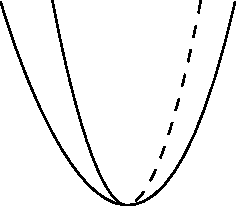
\includegraphics[width=8em]{figures/graph.pdf}
            \linebreak Graph mit $n=m=2$
        \end{minipage}

        Alternative $f(x,y) = -(x^{2}+y^{2}) \implies K(0) = 4$
        \item $f(x,y)= x^{n}-y^{n}$ mit $n,m \geq 2$
        \begin{align*}
            &(Hf)_{(x,y)}=\begin{pmatrix}
                n(n-1)x^{n-2} & 0\\ 0 & -m(m-1)y^{m-2}
            \end{pmatrix}\\
            &\implies K(0) = \begin{cases}
                0  &m\geq 3 \text{ oder } n \geq 3 \\
                -4  &m=n=2 
            \end{cases}\\
            &\text{Hier gilt }K(\varphi(u,v)) = \frac{-4}{(1+f_{u}^{2}+f_{v}^{2})^{2}} = -\frac{4}{(1+f_{u}^{2}+f_{v}^{2})^{2}} < 0\\
            &\text{Wir folgern } \lim\limits_{u\to\pm\infty}K(\varphi(u,v)) = 0 \text{, ebenso } \lim\limits_{v\to\infty}K(\varphi(u,v)) = 0.
        \end{align*}
    \end{enumerate}
\end{examples}
\begin{question}
    Existiert $f:\mathbb{R}^{2}\rightarrow\mathbb{R} \ C^{2}$, so dass $\Gamma_{f}$ konstant $-1$ gekrümmt ist?
\end{question}
\begin{answer}
    Nein! (Hilbert 1901)\\
    Im Spezialfall $f(x,y)=g(x)+h(y)$ mit $g,h:\mathbb{R}\to\mathbb{R} \ C^{2}$ können wir ``elementar'' zeigen, dass $\Gamma_{f}$ nicht konstant $-1$ gekrümmt sein kann (vergleiche Serie 6). 
    Mit der obigen Formel erhalten wir $$K(\varphi(u,v)) = \frac{g_{uu}\cdot h_{vv}}{(1+g_{u}^{2}+h_{v}^{2})^{2}} \stackrel{!}{=} -1$$
    $\implies g_{uu} \cdot h_{vv} < 0$\\
    \emph{Annahme:} $h_{vv} <0, g_{uu}> 0$ (für alle $(u,v)\in\mathbb{R}^{2}$ da $h,g$ stetig)\\
    Fixiere (ein beliebiges) $v \in\mathbb{R}$ und erhalte eine Differentialgleichung für $g$ der Form 
    $$ \frac{g_{uu}\cdot a}{(1+g_{u}^{2}+b^{2})} = -1 $$ mit $a = h_{vv}(v) < 0$ und $b=h_{v}(v)^{2}\geq 0$
    $$\implies g_{uu} = \underbrace{-\frac{1}{a}}_{>0 \text{ und } =:c} (1+g_{u}^{2}+b)^{2} = c\cdot (1+g_{u}^{2}+b)^{2} > c\cdot (1 + 2g_{u}^{2})$$
    Schreibe $s(u) = g_{u}(u) \implies s'>c(1+2s^{2})$ (evtl. reicht sogar $s'>2s^{2})$\\
    Wir lösen die Differentialgleichung $s' = c\cdot (1 + 2s^{2})$ und bemerken, dass diese in endlicher Zeit divergiert. 
\end{answer}
\begin{example}[nach Analysis 2]
    $s'=s^{2}$\\
    Lösung zur Anfangsbedingung: $s(0) = 1: s(t)=\frac{1}{1-t}$. Divergiert für $t\to 1$.
\end{example}
\pagebreak

\subsection*{Rotationsflächen}

\begin{minipage}{0.9\columnwidth}
    Sei $\gamma:\mathbb{R}\to\mathbb{R}^{2}$ eine $C^{2}$-Kurve. Schreibe $$\gamma(t) = (r(t),h(t))$$ mit $r(t)$ der Rotation und $h(t)$ der Höhe. Wir treffen folgende Annahmen:
    \begin{enumerate}
        \item $r(t)>0$
        \item $h'(t)>0$
        \item $||\dot{\gamma}(t)|| = 1$, d.h. $\dot{r}(t)^{2}+\dot{h}(t)^{2} = 1$ ("$\gamma$ ist nach Bogenlänge parametrisiert")
    \end{enumerate}
\end{minipage}
\vspace{0.05\linewidth}
\begin{minipage}{0.15\columnwidth}
    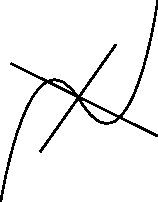
\includegraphics[width=5em]{figures/rotationsflaeche.pdf}
    \linebreak nicht erlaubt
\end{minipage}
\noindent
Konstruiere eine Rotationsfläche mit folgender Parametrisierung:\begin{align*}
    \varphi:\mathbb{R}\times(0,2\pi) &\to \Sigma\\
    (u,v) &\mapsto (r(u)\cos(v), r(u)\sin(v),h(u))
\end{align*}
Berechne \begin{align*}
    &\varphi_{u} = (r'(u)\cos(v), r'(u)\sin(v),h'(u))\\
    &\varphi_{v} = (-r(u)\sin(v), r(u)\cos(v), 0)
\end{align*}
Wir erhalten das folgende Einheitsnormalenfeld:
$$ N(\varphi(u,v)) = (-h'(u)\cos(v), -h'(u)\sin(v), r'(u))$$
Kontrolle:
\begin{itemize}
    \item $|| N || = 1$, d.h. $\langle N,N\rangle = 1$ (ok, da $h'(u)^{2}+r'(u)^{2}=1$)
    \item $\langle N,\varphi_{u}\rangle = 0$ (ok)
    \item $\langle N,\varphi_{v}\rangle = 0$ (ok)
\end{itemize}
Berechne \begin{align*}
    &E = \langle\varphi_{u},\varphi_{u}\rangle = 1 \text{ (da } h'^{2}+r'^{2}=1)\\
    &F = \langle\varphi_{u},\varphi_{v}\rangle = 0\\
    &G = \langle\varphi_{v},\varphi_{v}\rangle = r(u)^{2}
\end{align*}
Weiter \begin{align*}
    &e = \langle\varphi_{uu},N\rangle = h''(u)r'(u)-h'(u)r''(u)\\
    &f = \langle\varphi_{uv},N\rangle = 0\\
    &g = \langle\varphi_{vv},N\rangle = r(u)h'(u)
\end{align*}
\begin{align*}
    \implies K(\varphi(u,v)) &= \frac{eg-f^{2}}{EG-F^{2}} = \frac{(h''r'-h'r'')\cdot r\cdot h'}{r^{2}}\\
    &= \frac{1}{r}\cdot (h''r'h'-r''h'^{2}) = \frac{1}{r}\cdot (-r'^{2}r''-h'^{2}r'') = -\frac{r''(u)}{r(u)}
\end{align*}
Hierbei wurde genutzt, dass $r'^{2} + h'^{2} = 1 \implies 2r'r'' + 2h'h'' = 0$. 
Wir schliessen, dass $K(\varphi(u,v))$ nicht von $v$ abhängig ist!
\begin{specialcase}[Rotationsflächen mit konstanter Krümmung]
\leavevmode
\begin{enumerate}
    \item 
    \begin{minipage}[t]{0.8\columnwidth}
        $K=0$, d.h. $r''(u)=0$ $(\implies r(u)=a\cdot u+b)$.
        Anfangsbedingungen
        \begin{itemize}
            \item $r(0)=1$
            \item $r'(0)=0$
            \item $h(0)=0$
        \end{itemize}
        $\implies r(u)=1, h(u)=u$ mit $r'^{2}+h'^{2}=1$ und $h'>0 \implies h' = 1$\\
        Variation der Anfangsbedingung: $r'(0)=a \neq 0$ führt zu einem Kreiskegel:
        (Betrachte hier $\gamma:(x,+\infty)\rightarrow \mathbb{R}^{2}$ statt $\gamma:\mathbb{R}\rightarrow\mathbb{R}^{2})$
    \end{minipage}
    \hspace{0.05\linewidth}
    \begin{minipage}[t]{0.1\columnwidth}
        \begin{figure}[H]
            \centering
            \def\svgwidth{\textwidth}
            \input{figures/rotationsflaeche_1.pdf_tex}
        \end{figure}
    \end{minipage}

    \item
    $K=1$, d.h. $r''=-r$
    Anfangsbedingungen
    \begin{itemize}
        \item $r(0)=1$
        \item $r'(0)=0$
        \item $h(0)=0$
    \end{itemize}
    $\implies r(u)=\cos(u), h(u)=\sin(u)$. Einheitsspähre $S^2$.
    Variation der Anfangsbedingung führt zu vertikal verschobenen Einheitssphären, oder keiner Lösung;
    \begin{example}
        $r(0)=2, \ r'(0)=0, \ h(0)=0 \implies$
        \begin{itemize}
            \item $r(u)=2\cos(u)$
            \item $h(u)=\int_{0}^{u} h'(x) dx = \int_{0}^{u} \sqrt{1-4(\sin(x))^{2}} dx$
        \end{itemize}
        mit $r'^{2}+h'^{2}=1$, hierbei handelt es sich um ein elliptisches Integral, nicht ausdrückbar durch elementare Funktionen.
        \begin{figure}[H]
            \centering
            \def\svgwidth{\textwidth}
            \input{figures/rotationsflaeche_2.pdf_tex}
        \end{figure}
    \end{example}
    \item $K=-1$, d.h. $r'' = r$.
    Anfangsbedingungen
    \begin{itemize}
        \item $r(0)=1$
        \item $r'(0)=0$
        \item $h(0)=0$
    \end{itemize}
    $\implies r(u)=\frac{1}{2}(e^{u}+e^{-u})=\cosh(u),\ h(u)=\dots$ \\ \noindent Es gilt:
    $$r'(u)=\cosh(u)'=\sinh(u)=\frac{1}{2}(e^{u}-e^{-u}) \overset{u \to \pm \infty}{\longrightarrow} \pm \infty$$
    Folglich existiert auch hier die Fläche $\Sigma$ nur über einem gewissen Interval der Form $(-h_{0},h_{0})$. (vgl. Serie 7)
    \begin{figure}[htb]
        \centering
        \def\svgheight{6em}
        \input{figures/rotationsflaeche_3.pdf_tex}
    \end{figure}
\end{enumerate}
\end{specialcase}



\section{Theorema Egregium}
\begin{goal}
    Die Krümmung ist durch die Koeffizientenfunktionen $E,F,G$ bestimmt. Genauer: durch $E,F,G$ und ihre Ableitungen bestimmt.
\end{goal}
Sei $\varphi:U\to V \subset \Sigma$ eine lokale $C^{2}$-Parametrisierung und $N:V\to S^{2}$ die zugehörige lokale Gaussabbildung.
Für alle $p\in V$ gilt. $$K(p) = \det(DN)_{p} = \frac{eg-f^{2}}{EG-F^{2}}$$
Matrix von $(DN)_{p}:T_{p}\Sigma\to T_{p}\Sigma$ bezüglich der Basis $$\{\varphi_{u},\varphi_{v}\}: \begin{pmatrix}
    a_{11} & a_{12}\\ a_{21} & a_{22} \end{pmatrix}$$ dass heisst \begin{align*}
        N_{u} &= (DN)_{\varphi(u,v)}(\varphi_{u}) = a_{11} \varphi_{u} + a_{21}\varphi_{v}\\
        N_{v} &= (DN)_{\varphi(u,v)}(\varphi_{v}) = a_{12} \varphi_{u} + a_{22}\varphi_{v}
    \end{align*}
Es gilt: $e = \langle\varphi_{uu}, N\rangle, f = \langle\varphi_{uv}, N\rangle, g = \langle\varphi_{vv}, N\rangle$ und wir folgern: $$\varphi_{uu}-eN\perp N\\ \implies \varphi_{uu}-eN \in \spann{\{\varphi_{u},\varphi_{v}\}}$$
Ähnlich existieren eindeutige Koeffizienten $\Gamma_{11}^{1},\Gamma_{11}^{2},\Gamma_{12}^{1},\Gamma_{12}^{2},\Gamma_{22}^{1},\Gamma_{22}^{2}\in\mathbb{R}$ sogenannte Christoffelsymbole, mit \begin{align*}
    \varphi_{uu} &= eN + \Gamma_{11}^{1}\cdot\varphi_{u} + \Gamma_{11}^{2}\cdot\varphi_{v}\\
    \varphi_{uv} &= fN + \Gamma_{12}^{1}\cdot\varphi_{u} + \Gamma_{12}^{2}\cdot\varphi_{v}\\
    \varphi_{vv} &= gN + \Gamma_{22}^{1}\cdot\varphi_{u} + \Gamma_{22}^{2}\cdot\varphi_{v}
\end{align*} Berechne nun $$\langle\varphi_{uu},\varphi_{u}\rangle = \frac{1}{2}\left(\frac{\partial}{\partial u}(\langle\underbrace{\varphi_{u},\varphi_{u}}_{=E}\rangle)\right) = \frac{1}{2}E_{u}$$ und 
$$\langle\varphi_{uu},\varphi_{v}\rangle = \frac{\partial}{\partial u}\langle\underbrace{\varphi_{u},\varphi_{v}}_{=F}\rangle - \langle\varphi_{u},\varphi_{uv}\rangle = F_{u} - \frac{1}{2}E_{v} \qquad \left(\frac{\partial}{\partial v}\langle\varphi_{u},\varphi_{u}\rangle = 2\cdot\langle\varphi_{u},\varphi_{vu}\rangle\right)$$
Anderseits gilt nach obrigen Ansatz für $\varphi_{uu},\varphi_{uv},\varphi_{vv}$ auch \begin{align*}
    \langle\varphi_{uu},\varphi_{u}\rangle &= \Gamma_{11}^{1}\cdot E + \Gamma_{11}^{2}\cdot F\\
    \langle\varphi_{uu},\varphi_{v}\rangle &= \Gamma_{11}^{1}\cdot F + \Gamma_{11}^{2}\cdot G
\end{align*} die Gleichheiten folgt jeweils aus $\langle N,\varphi_{u}\rangle$
$$\implies \begin{pmatrix}
    E&F\\F&G
\end{pmatrix}\cdot \begin{pmatrix}
    \Gamma_{11}^{1}\\\Gamma_{11}^{2}
\end{pmatrix} = \begin{pmatrix}
    \frac{1}{2} E_{u}\\ F_{u}-\frac{1}{2}E_{v}
\end{pmatrix}$$
Analog erhalten wir via $\varphi_{uv}$ und $\varphi_{vv}$ \begin{itemize}
    \item $\begin{pmatrix}
        E&F\\F&G
    \end{pmatrix}\cdot\begin{pmatrix}
        \Gamma_{12}^{1}\\\Gamma_{12}^{2}
    \end{pmatrix} = \begin{pmatrix}
        \frac{1}{2}E_{v}\\\frac{1}{2}G_{u}
    \end{pmatrix}$
    \item $\begin{pmatrix}
        E&F\\F&G
    \end{pmatrix}\cdot\begin{pmatrix}
        \Gamma_{22}^{1}\\\Gamma_{22}^{2}
    \end{pmatrix} = \begin{pmatrix}
        F_{v}-\frac{1}{2}G_{u}\\\frac{1}{2}G_{v}
    \end{pmatrix}$
\end{itemize} Beachte hier: $\det{\begin{pmatrix}
    E&F\\F&G
\end{pmatrix}} = EG-F^{2} > 0$, da $I_{p}$ positiv definit ist.
\begin{consequence}
    Die $\Gamma_{ij}^{k}$ sind durch $E,F,G$ und ihre partiellen Ableitungen bestimmt.\\
    $K$ ist durch $E,F,G$ bestimmt.
\end{consequence}
\begin{recall}
    \begin{align*}
        \varphi_{uu} &= eN+\Gamma_{11}^{1}\varphi_{u} + \Gamma_{11}^{2}\varphi_{v}\\
        \varphi_{uv} &= fN+\Gamma_{12}^{1}\varphi_{u} + \Gamma_{12}^{2}\varphi_{v}\\
        \varphi_{vv} &= gN+\Gamma_{22}^{1}\varphi_{u} + \Gamma_{22}^{2}\varphi_{v}
    \end{align*}
\end{recall}
Via $\langle\varphi_{uu},\varphi_{u}\rangle$ etc, erhalten wir $\Gamma_{ij}^{k}$ als Funktion von $E,F,G$ und ihren ersten partiellen Ableitungen.
\begin{lemma}
    Sei $\varphi:U\to V\subset\Sigma$ eine lokale $C^{3}$-Parametrisierung. Dann gilt $\forall p\in V:$
    $$-E K = (\Gamma_{12}^{2})_{u}-(\Gamma_{11}^{2})_{v}+\Gamma_{12}^{1}\cdot\Gamma_{11}^{2}+\Gamma_{12}^{2}\cdot\Gamma_{12}^{2}-\Gamma_{11}^{2}\cdot\Gamma_{22}^{2}-\Gamma_{11}^{1}\cdot\Gamma_{12}^{2}$$
\end{lemma}
\begin{corollary}[Theorema Egregium, Gauss 1827]
    Die Krümmung $K$ lässt sich durch $E,F,G$ und deren zwei partiellen Ableitungen ausdrücken.
\end{corollary}
\begin{proof}[Beweis des Korollars]
    Es gilt $E=\langle\varphi_{u},\varphi_{u}\rangle > 0$ da $I_{p}:T_{p}\Sigma\to\mathbb{R}$ positiv definit ist.
    $$\implies K = -\frac{1}{E}(\dots)$$ wobei die $\dots$ ein Ausdruck in $\Gamma_{ij}^{k}$ und erste partielle Ableitungen, also Ausdruck in $E,F,G$ und zweite partielle Ableitungen sind.
\end{proof}
\begin{remark}
    Das Korollar gilt auch für Flächen der Regularität $C^{2}$.
\end{remark}
\begin{proof}[Beweis Lemma]
    Wir berechnen $\varphi_{vuu}=\varphi_{uuv}$ \begin{enumerate}
        \item $$\varphi_{vuu} = \frac{\partial}{\partial v}(\varphi_{uu}) = e_{v}N+e\underbrace{N_{v}}_{a_{12\varphi_{u}+a_{22}\varphi_{v}}}+(\Gamma_{11}^{1})_{v}\varphi_{u}+\Gamma_{11}^{1}\varphi_{vu}+(\Gamma_{11}^{2})_{v}\varphi_{v}+\Gamma_{11}^{2}\varphi_{vv}$$
        \item $$\varphi_{uuv} = \frac{\partial}{\partial u}(\varphi_{uv}) = f_{u}N+f\underbrace{N_{u}}_{a_{11\varphi_{u}+a_{21}\varphi_{v}}}+(\Gamma_{12}^{1})_{u}\varphi_{u}+\Gamma_{12}^{1}\varphi_{uu}+(\Gamma_{12}^{2})_{u}\varphi_{v}+\Gamma_{12}^{2}\varphi_{uv}$$
    \end{enumerate}
    Die $\varphi_{v}$-Komponente von $\varphi_{vuu}$ und $\varphi_{uuv}$ ist gleich, also 
    $$e\cdot a_{22}+\Gamma_{11}^{1}\Gamma_{12}^{2}+(\Gamma_{11}^{2})_{v}+\Gamma_{11}^{2}\Gamma_{22}^{2} = f\cdot a_{21}+\Gamma_{12}^{1}\Gamma_{11}^{2}+(\Gamma_{12}^{2})_{u}+\Gamma_{12}^{2}\Gamma_{12}^{2} \ \ (*)$$
    (Benutze $\varphi_{uv} = fN+\Gamma_{12}^{1}\varphi_{u}+\Gamma_{12}^{2}\varphi_{v}$, etc.)
    \begin{recall}
        \begin{align*}
            &\begin{pmatrix}
                a_{11}&a_{21}\\a_{12}&a_{22}
            \end{pmatrix} \begin{pmatrix}
                E&F\\F&G
            \end{pmatrix} = -\begin{pmatrix}
                e&f\\f&g
            \end{pmatrix}\\
            &\implies \begin{pmatrix}
                E&F\\F&G
            \end{pmatrix} = -(a_{ij})^{-1}\begin{pmatrix}
                e&f\\f&g
            \end{pmatrix} \underset{K = \det(a_{ij})}{=} -\frac{1}{K}\begin{pmatrix}
                a_{22}&-a_{21}\\-a_{12}&a_{11}
            \end{pmatrix} \begin{pmatrix}
                e&f\\f&g
            \end{pmatrix}\\
            &\implies E = -\frac{1}{K} (a_{22}e-a_{21}f)\\
            &\text{bzw. } -E K = a_{22}e-a_{21}f \qquad \text{ (gilt auch für } K=0 \text{)}\\
            &\implies -E K \overset{(*)}{=} 6 \text{ Terme in } \Gamma_{ij}^{k} \text{ (siehe Lemma)}
        \end{align*}
    \end{recall}
\end{proof}
\begin{remark}
    Ähnliche Ausdrücke erhalten wir für $-F K$ und $-G K$.
\end{remark}
\end{document}